\section{Experiments}
\label{sec:results}

\begin{table*}[t]
\centering
\footnotesize
\setlength{\tabcolsep}{4.5pt}
\begin{tabular}{@{}lccccc@{}}
\toprule
& \multicolumn{3}{c}{cross-FSC, half 1 / half 2} & 5L93 FSC 0.5 & wall clock \\
\cmidrule(lr){2-4}
Method & 0.143 crossing (\AA) $\downarrow$ & at 3.5\,\AA\ $\uparrow$ & mean 3.6--3.28\,\AA\ $\uparrow$ & (\AA) $\downarrow$ & from picks (h) \\
\midrule
% rows generated by scripts/paper_figures_cvpr.py (tab_benchmark) from the score directories named in each % src line
\csname @@input\endcsname fig/tab_benchmark_rows.tex
\bottomrule
\end{tabular}
\caption{\textbf{End-to-end benchmark on EMPIAR-10164} (9,038 particles, C6), every map scored by the same scorer.
Columns 2--4: each STAGS half map against the opposite RELION-5 polished half map, inside RELION's mask, with phase-randomization mask correction; the RELION-5 rows score their own half maps the same way, so the polished row is RELION's half-map FSC.
Column 5: average of the two normalized half maps against the deposited model 5L93.
STAGS times: one wall clock on $2\times$ RTX PRO 6000 Blackwell, initial particle picks to final map.
$^\dagger$4.33\,h including initial extraction and completion of the background scoring.
% src: runs/engine/pose_abc_adopt_20261113/blind/wall_clock.json (wall_min 259.49)
$^\ddagger$Cumulative times in the RELION-5 project's own logs, other hardware; the RELION-5 paper reports 13\,h\,04\,min from the picks to its first bin-1 map and 3\,h\,22\,min per polishing round on $2\times$ RTX 4090~\cite{burt2024relion5}.
% src: docs/relion5-paper-table4.md
The earlier STAGS runs used the recipe before the pose corrections of \cref{sec:results:ablation} and other code revisions.}
\label{tab:benchmark}
\end{table*}


\subsection{Setup}
\label{sec:results:setup}

\paragraph{Data and baselines.}
We use EMPIAR-10164, the RELION-5 tomography tutorial~\cite{iudin2023empiar,burt2024relion5}: immature HIV-1 CA-SP1 hexamers~\cite{schur2016hiv} (C6) in five tilt series, 9,038 particles in RELION's half-sets of 4,536 and 4,502.
% src: runs/engine/pose_abc_adopt_20261113/completion_review.json (recipe_checks: 4536/4502 particles)
STAGS starts from the initial picks with the pre-refinement tilt alignment and CTF; a file guard verified that it opened no refined RELION file.
% src: scripts/engine_inputs.py (docstring); runs/engine/pose_abc_adopt_20261113/blind/report.json (guard passed, 0 violations)
It inherits RELION's final particle selection and half-sets, and one scalar, the volume of RELION's mask (315,397 voxels), shapes its own masks.
% src: scripts/engine_inputs.py (Select/job077 traced to Extract/job010); blind/launch.json (mask_volume_prior.voxels 315397)
Baselines are the stored RELION-5 maps after auto-refinement and after five rounds of CTF refinement, Bayesian polishing~\cite{zivanov2019polishing} and refinement (``polished''), at the cumulative times in the project's logs (12.4 and 24.1\,h, other hardware).
% src: scripts/lean_chain.py (RELION hours 12.43, 24.1); docs/relion5-paper-table4.md
STAGS runs on $2\times$ RTX PRO 6000 Blackwell, one half-set per GPU.
% src: CLAUDE.md (KW61627); blind/launch.json (host KW61627)

\paragraph{Metrics.}
One scorer evaluates every map on RELION's $192^3$, 1.35\,\AA\ grid, inside RELION's mask, with phase-randomization correction~\cite{chen2013highres}.
% src: runs/engine/pose_abc_adopt_20261113/blind/scores/cycle4/structure/results.json (protocol)
The \emph{cross-FSC}~\cite{rosenthal2003fsc} compares each STAGS half map with the \emph{opposite} RELION-5 polished half map; we report its 0.143 crossing, its value at 3.5\,\AA\ and its mean over the eight shells from 3.6 to 3.28\,\AA.
% src: blind/comparison.json (band_definition: native shells 72-79, equal weights)
RELION's maps are scored the same way, so the polished row is RELION's own half-map FSC.
Atomic agreement is the FSC~0.5 crossing of the half-map average against the deposited model 5L93~\cite{schur2016hiv}.
These scores are reference-assisted.
STAGS's own half-map FSC stays above 0.143 up to Nyquist (0.61 at 3.5\,\AA) and is not used as a resolution estimate.
% src: blind/scores/cycle4/results.json (table.gold: cross_0143 null, fsc["3.5"] = 0.610)

\subsection{End-to-end benchmark}
\label{sec:results:benchmark}

\Cref{tab:benchmark} and \cref{fig:teaser} report one fresh run from the picks, which stopped itself after four refinement cycles when the median rotation update fell below its threshold.
% src: runs/engine/pose_abc_adopt_20261113/completion_review.json (stopping medians 0.379/0.380 deg < 0.401 deg)
Its cross-FSC crosses 0.143 at 3.269 and 3.251\,\AA, against 3.284\,\AA\ for the polished map and 3.65/3.63\,\AA\ for auto-refinement.
% src: blind/comparison.json; tab_benchmark_rows.tex (job023 3.646/3.632)
The polished map remains ahead in the band just above the crossing (mean FSC 0.244 against 0.228/0.226) and in atomic agreement (3.86 against 4.04\,\AA).
% src: blind/comparison.json (band means; atomic_merged_fsc05_A)
The crossing margins (0.014/0.033\,\AA) come from a single run and are smaller than the spread of earlier STAGS runs, so we read them as parity.
% src: completion_review.json (gain_vs_RELION_crossing_A); tab_benchmark_rows.tex (runs C/D/E 3.343-3.414)
The run took 4.27\,h from the picks to the final map (4.33\,h including extraction and scoring): 89\,min of coarse-to-fine levels, a 19\,min map fit and 35--37\,min per refinement cycle.
% src: blind/report.json (wall_min 256.23); wall_clock.json (259.49); run_abc.log (ladder 89.2 min; KB fit 19.4 min; cycles 37.1/35.9/35.4/34.6 min)
This is 18\,\% of RELION's logged 24.1\,h, but not a same-hardware comparison; the RELION-5 paper reports 13\,h before polishing on $2\times$ RTX 4090~\cite{burt2024relion5}.
% src: 4.33/24.1 = 0.18; docs/relion5-paper-table4.md (13 h 04 min)
The final recipe includes three pose corrections that were adopted after their predeclared gate had failed (\cref{sec:results:ablation}).

\begin{figure*}[t]
\centering
% src: fig/abc_fsc.png by scripts/paper_figures_abc.py; curves: docs/paper/fig_abc_fsc.csv; crossings: docs/paper/fig_abc_provenance.json (fsc_crossings_A)
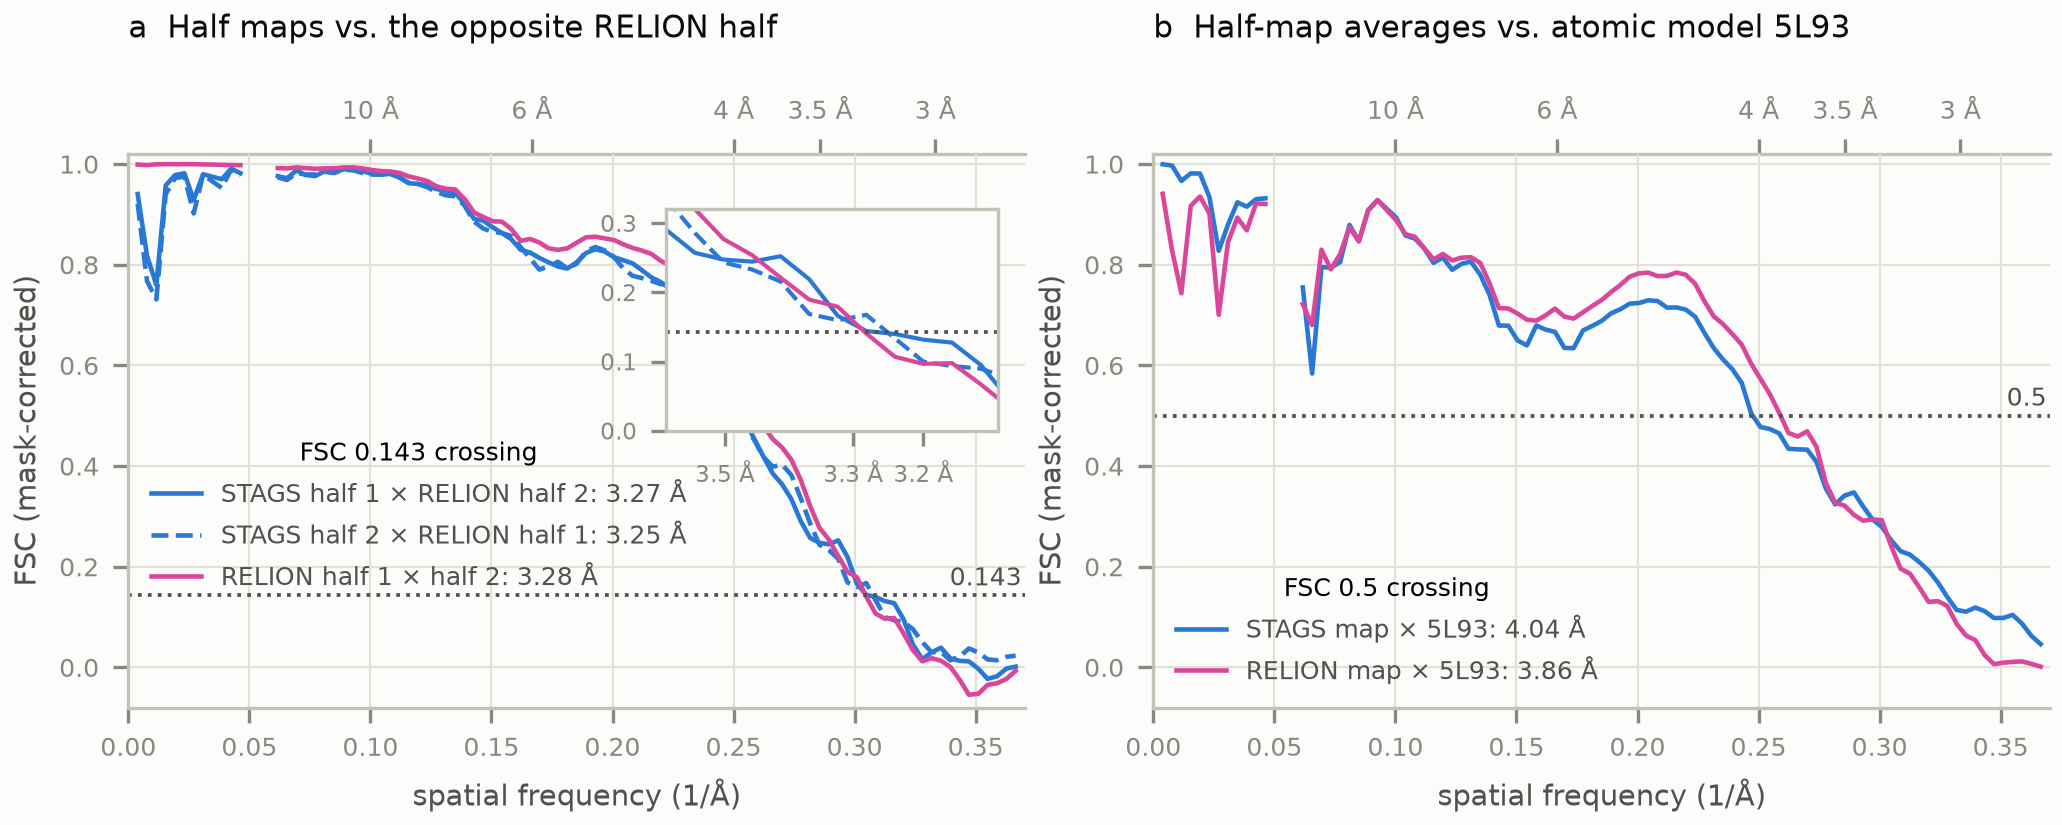
\includegraphics[width=\textwidth]{fig/abc_fsc.png}
\caption{\textbf{Fourier shell correlation, STAGS versus the RELION-5 polished map.}
(a)~Each STAGS half map against the opposite RELION-5 half map (blue; 3.27 and 3.25\,\AA\ at FSC~0.143) and RELION's own half 1 against half 2 (magenta; 3.28\,\AA); inset, 3.6--3.1\,\AA.
(b)~Average of the two normalized half maps against the atomic model 5L93: STAGS 4.04\,\AA, RELION-5 3.86\,\AA\ at FSC~0.5.
All curves: maps registered on RELION's $192^3$, 1.35\,\AA\ grid, RELION's mask, phase-randomization correction beyond 20\,\AA; gaps near 20\,\AA\ are the correction's transition shells, which the scorer leaves undefined.}
\label{fig:fsc}
\end{figure*}


\subsection{Side-by-side comparison}
\label{sec:results:visual}

\Cref{fig:fsc,fig:closeups,fig:locres} compare the two maps under identical processing; the supplement adds rendered views and central sections (\cref{sec:suppl:visual}).
Both STAGS cross-FSC curves follow RELION's half-map FSC through the crossing (\cref{fig:fsc}a).
Against the atomic model, STAGS is lower from about 8 to 3.6\,\AA, by up to 0.10 (\cref{fig:fsc}b), and RELION's close-ups show sharper side-chain protrusions (\cref{fig:closeups}).
% src: docs/paper/fig_abc_fsc.csv (difference -0.099 at 4.05 A; negative 8.1-3.55 A); docs/final-campaign-nov13.md (Visual comparison)
With one local-resolution estimator for both maps (\cref{fig:locres}), the median is 3.26\,\AA\ for RELION's own halves and 3.20\,\AA\ for the STAGS halves against RELION's; windows coarser than 4\,\AA\ (13\,\% for RELION, 8\,\% for STAGS) lie mostly within 10\,\AA\ of the mask boundary.
% src: docs/paper/fig_abc_provenance.json (local_resolution.summary: median 3.2589 / 3.2005; fraction_coarser_than_4A 0.133 / 0.075; coarse_within_10A_of_mask_edge 0.72 / 0.79 vs all windows 0.48)
Because STAGS is scored against RELION's halves, this measures agreement with RELION, not the independent local resolution of the STAGS map.

\begin{figure*}[t]
\centering
% src: fig/abc_closeups.png by scripts/paper_figures_abc.py; regions: docs/paper/fig_abc_fig6c_regions.json; leads: docs/final-campaign-nov13.md (Visual comparison)
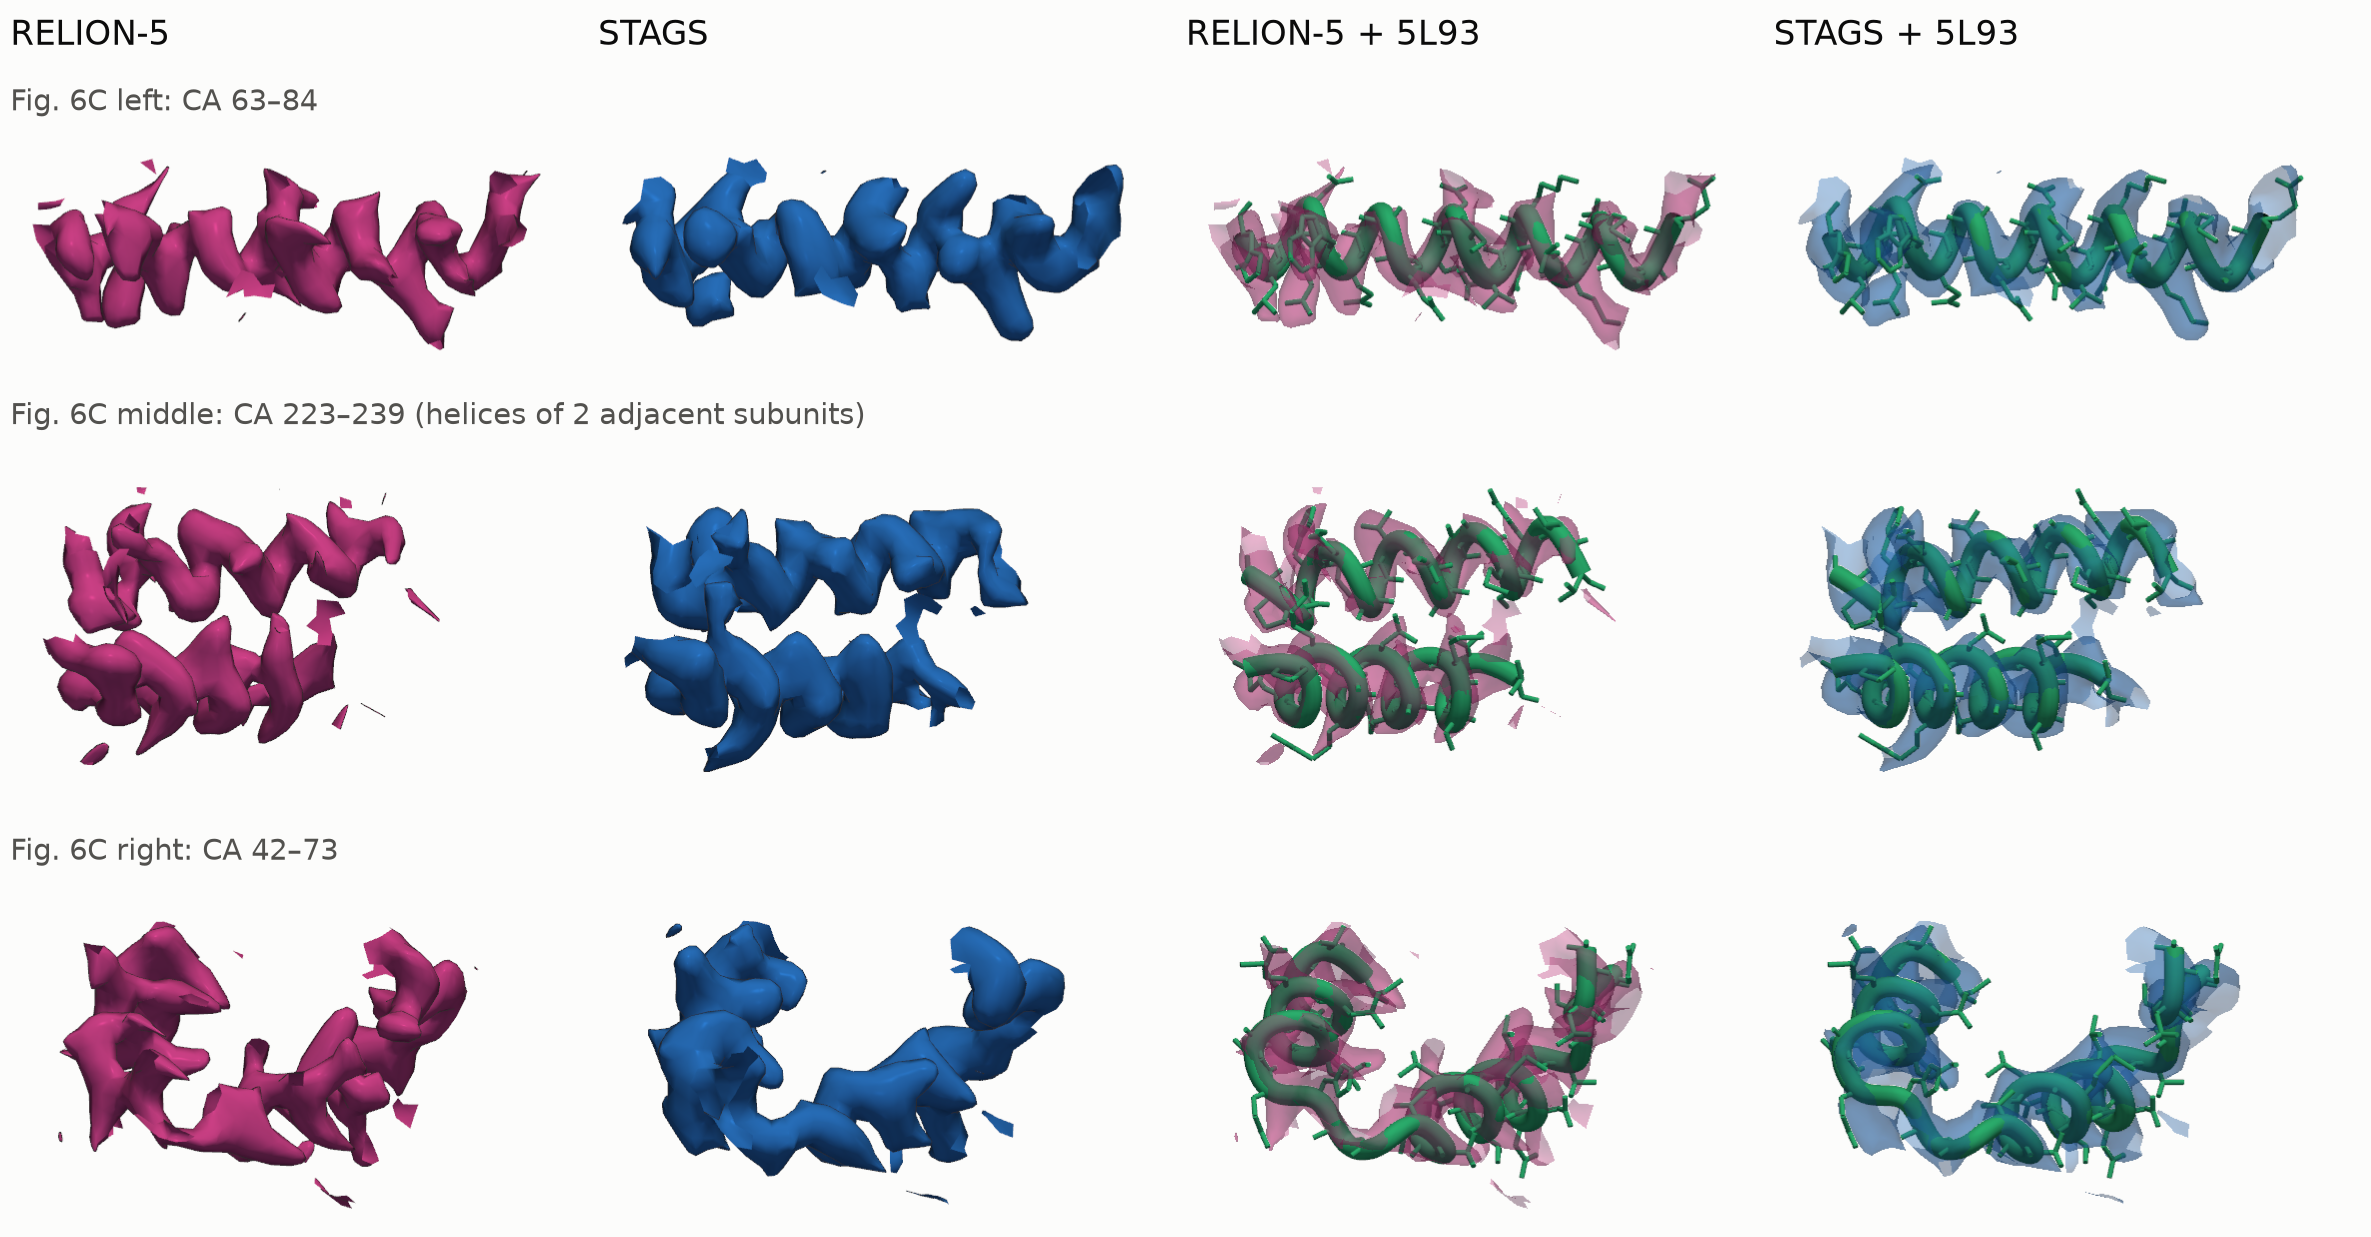
\includegraphics[width=0.92\textwidth]{fig/abc_closeups.png}
\caption{\textbf{Close-ups of the three regions shown in RELION-5's Fig.~6C~\cite{burt2024relion5}.}
Columns: RELION-5 polished map, STAGS, then each map translucent over the 5L93 model.
Rows: CA residues 63--84 (helix~4); 223--239 of two adjacent subunits; 42--73 (end of helix~2 to the start of helix~4).
The published figure does not list its regions; we recovered them by a joint silhouette match of 5L93 atoms and RELION density to the published panels, with leads of 1.59, 0.71 and 0.46\,px over the next distinct region, so the bottom row is the least certain.
Same filtering and threshold as \cref{fig:views}, zoned 2.5\,\AA\ around the shown residues, identical camera per row.}
\label{fig:closeups}
\end{figure*}

\begin{figure*}[t]
\centering
% src: fig/abc_locres.png by scripts/paper_figures_abc.py (render --paper); numbers: docs/paper/fig_abc_provenance.json (local_resolution); docs/paper/fig_abc_locres.csv
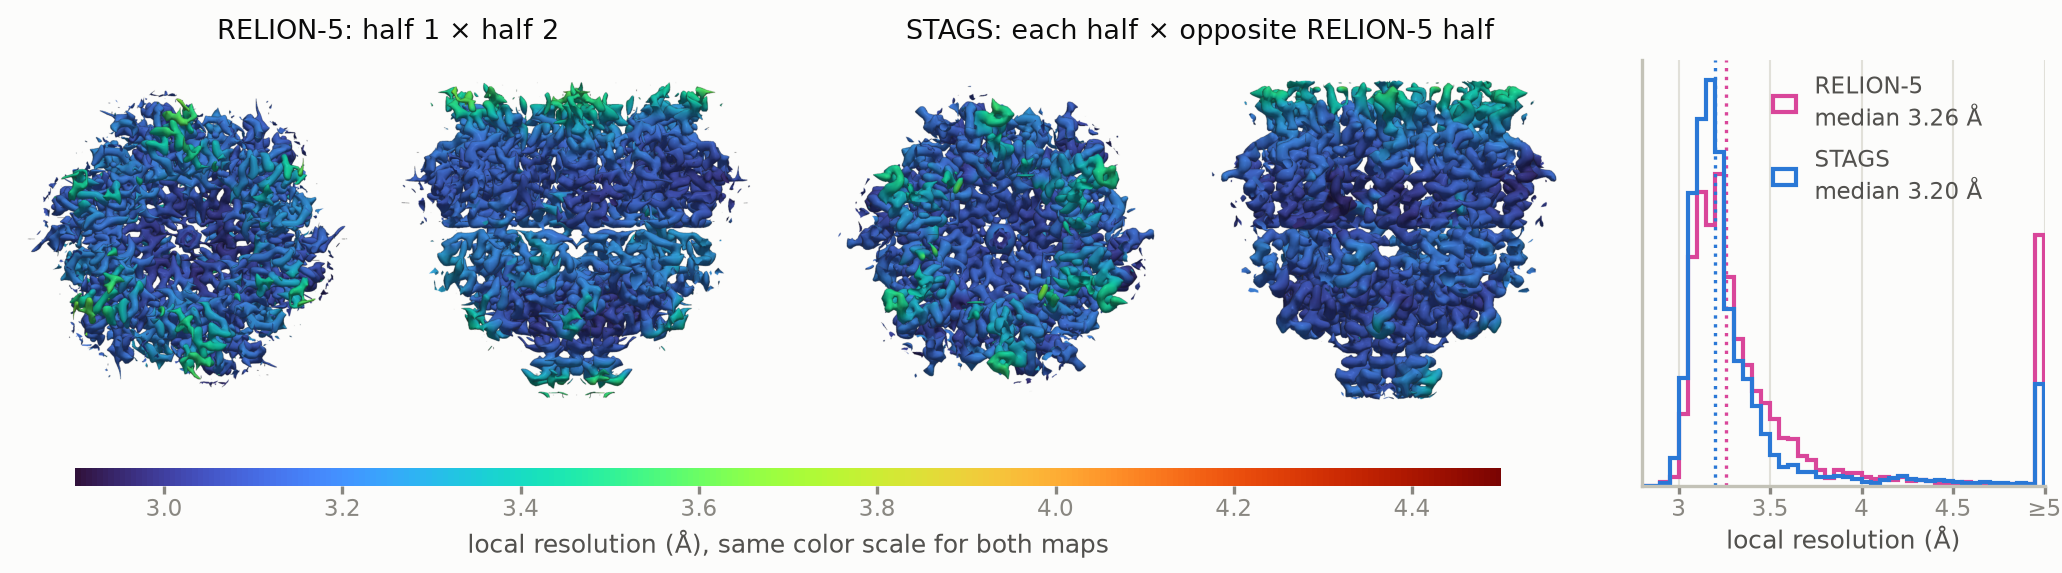
\includegraphics[width=\textwidth]{fig/abc_locres.png}
\caption{\textbf{Local resolution with one estimator for both maps.}
Top and side views of the central hexamer (surfaces as in the supplementary \cref{fig:views}), colored on one scale by windowed FSC~0.143 (40\,px box, cosine sphere from 10.8 to 18.9\,\AA, every 3\,px, phase-randomization correction beyond 20\,\AA); right, the distribution over all window centers inside RELION's mask.
RELION-5: its half 1 against half 2 (median 3.26\,\AA).
STAGS: each half against the opposite RELION-5 half (median 3.20\,\AA), which measures agreement with RELION, because STAGS's own half maps stay above FSC~0.143 up to Nyquist.}
\label{fig:locres}
\end{figure*}


\subsection{Fixed-pose particle efficiency}
\label{sec:results:efficiency}

\begin{table}[t]
\centering
\footnotesize
\setlength{\tabcolsep}{3.5pt}
\resizebox{\columnwidth}{!}{%
\begin{tabular}{@{}lccccc@{}}
\toprule
& voxel & Gaussian & map-only & voxel & 5L93 FSC 0.5 (\AA) \\
Withheld & 250 & 250 & 250 & 500 & voxel / Gaussian 250 \\
\midrule
% rows generated by scripts/paper_figures_cvpr.py (tab_efficiency); per-row % src lines inside
\csname @@input\endcsname fig/tab_efficiency_rows.tex
\bottomrule
\end{tabular}}
\caption{\textbf{Fixed-pose reconstruction at equal particle counts.}
Mean mask-corrected FSC against the RELION-5 polished half-2 map over 6.5--5.6\,\AA\ ($\uparrow$); RELION's refined poses, optics and mask throughout.
(i)~250 half-1 particles from four tomograms, the fifth withheld; voxel maps by RELION-5 (500: nested superset); map-only: Gaussians fitted to the voxel-250 map (primary split only).
(ii)~Five disjoint draws, 200 particles reserved, ridge-regularized voxel solver; details in \cref{sec:suppl:efficiency}.}
\label{tab:efficiency}
\end{table}


To isolate the representation, we fix RELION's refined poses, optics and mask and compare Gaussians fitted to the particle images with voxel reconstruction from the same particles (\cref{tab:efficiency}).
Three predeclared splits each train on 250 half-1 particles from four tomograms and withhold the fifth for image prediction; the voxel baseline is RELION-5's reconstruction.
% src: runs/native_limited250_20261103/selection.json; docs/stags-limited-particle-study-matrix.md (replications hold out TS03, TS45)
In every split the Gaussian map agrees better with the half-2 map (mean FSC over 6.5--5.6\,\AA\ +0.061, +0.086, +0.057) and with 5L93.
% src: docs/results-limited250-three-study-20261103.md; runs/native_limited250_{20261103,R1_20261104,R2_20261104}/native500_score/results.json
Fitting the same Gaussian initialization and schedule to the 250-particle voxel map instead of the images gives 0.508, the voxel map's level (0.509) rather than 0.570, which attributes the gain to the image-level fit.
% src: runs/native_limited250_20261103/control_v4_outcome.json; map_only_control_v4/score/results.json
These results carry qualifications (\cref{sec:suppl:efficiency}).
The predeclared Gaussian arms, fitted to raw images, failed (0.243 against 0.509); the reported recipe is an earlier one, substituted after that failure and scored under the same frozen gates.
% src: docs/results-limited250-primary-20261103.md (ray250 0.243, native 0.509); runs/step2_parity_20261103/decision.json
RELION-5 with 500 particles remains better in every split.
The map-only control ran once and does not reproduce the voxel map (earlier versions missed the required relative $L_2$ error of 0.10).
% src: runs/native_limited250_20261103/{map_only_control/decision.json,controls_v2_outcome.json,control_v3_outcome.json}
Image prediction on the withheld tomogram barely separates the methods (differences below 0.1\,\% of the observed power).
% src: native500_score/results.json (loss_over_observed_power); docs/results-limited250-primary-20261103.md
A second study with five disjoint draws points the same way (\cref{tab:efficiency}, ii).
% src: runs/particle_efficiency_20261102/results.json

\subsection{Ablations}
\label{sec:results:ablation}

Three pose corrections were tested in matched one-cycle continuations from the final state of an earlier run (\cref{sec:suppl:ablation}): exact Fourier-phase translation scoring, a masked Gaussian search reference, and separate static and shared motion in polishing.
Each alone gained at most 0.021\,\AA; together they gained 0.082\,\AA\ on half~1 but 0.015\,\AA\ on half~2, failing the predeclared gate of $>0.03$\,\AA\ on each half.
% src: runs/engine/posefix_20261113/{a,b,c,abc}/result.json; engine_rules.json steps.posefix_20261113
We adopted the combination after seeing these results, because its band-mean FSC rose on both halves (+0.016/+0.017); the failed gate stands.
% src: docs/final-campaign-nov13.md (Explicit post-result adoption)
